\section{Análisis estructural}
Una estrategia para poder analizar el funcionamiento y estructura del modelo es analizar la
cantidad de mensajes enviados por cada uno de sus componentes (modelos atómicos o acoplados). 
Esto nos permite ver los valores de salida emitidos por los modelo, de transiciones internas o eventos
externos.

Este tipo análisis, junto con uno de tiempos de ejecución, puede servir para comparar modelos equivalentes, a fin de determinar que implementación conviene utilizar a medida que se complejizan los experimentos y/o modelos compuestos. En este caso, podríamos comparar el modelo donde los \textit{stocks} son acoplados del modelo aplanado.

Para un modelo sencillo como el de la taza de té generamos gráficos que nos
permiten analizar el comportamiento de la simulación en dos ejes, los eventos
realizados por cada atómico o el acoplado \texttt{top}.

Para poder generar este, categorizamos cada línea de \textit{log} para cada modelo y
contamos su frecuencia. Luego, agrupamos estos datos y generamos un Heatmap.
Este gráfico nos permite visualizar las dimensiones \textit{modelo}, \textit{tipo de mensaje} y
\textit{cantidad de ocurrencias} para poder compararlos entre sí.

Dado que el \texttt{TopLevelCoupled} (\texttt{TLC})  es el orquestador de la simulación,
observamos mayor cantidad de eventos de tipo \textit{@, Done e Y}. La alta
frecuencia de eventos \textit{Y} se explica sabiendo que éste  transporta la
información de salida. Dada la diferencia de magnitudes entre los distintos
modelos utilizamos una escala logarítmica y una escala lineal para analizar los
datos.

En la figura \ref{fig:teacup_cant_mensajes} observamos la  ejecución del modelo
de enfriamiento de una taza de té. En el eje de las $X$ tenemos los mensajes 
y en el eje de las $Y$ tenemos los distintos modelos. 
Esta figura se generó a partir de los datos simulados con el modelo traducido.
Podemos observar que para los modelos $FTot$, $FMinus$ e $Integrador$ la cantidad 
de transiciones internas, externas y de salida son iguales. Esto es razonable 
debido a que estos 3 modelos generan un ciclo entre sí, es decir que se retroalimentan.

Para poder analizar el comportamiento de las salidas de cada modelo, utilizamos
un gráfico de tipo \textit{Letter Value} que puede observarse en \ref{fig:teacup_output_letter_plot}.
Éste nos indica además de los estadísticos principales (media, percentiles y outliers), 
la densidad de los valores que se encuentran en un rango de la muestra. 
Por ejemplo podemos ver que la muestra está no solo centrada en los 115 grados sino que 
más del 50\% de dichos valores se encuentran allí. 

En esta figura se observa claramente como los modelos de \textit{FTot} y \textit{FMinus} 
arrojan valores de out con un rango de valores acotado centrados alrededor del cero. 
En el caso del integrador que es el que calcula los valores de temperatura de la taza, 
es razonable ver que los valores van desde los 180 grados a los 70. Se observa también 
la alta densidad de valores entre los 90 y los 135 grados. Los valores por debajo de los 
70 pueden tener que ver con el método de integración. 

Para mayor legibilidad quitamos los valores del modelo \textit{characteristictime} 
ya que este era constante y no aportaba al análisis.

\begin{figure}[H]
    \centering     %%% not \center
    \subfigure[Cantidad mensajes modelo teacup]{\label{fig:teacup_cant_mensajes}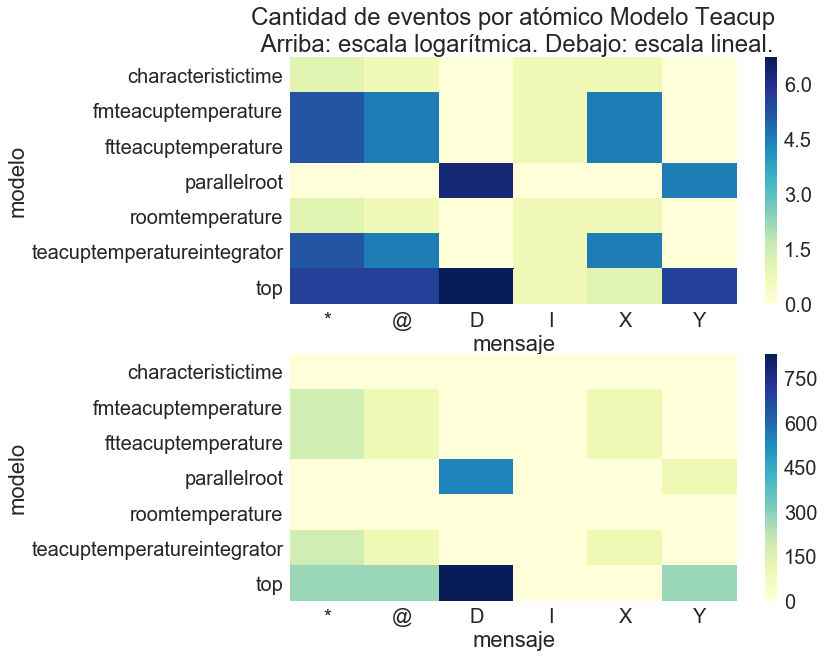
\includegraphics[scale=0.4]{imagenes/tea_cantidad_mensajes}}
        \subfigure[Valores de salida modelo teacup]{\label{fig:teacup_output_letter_plot}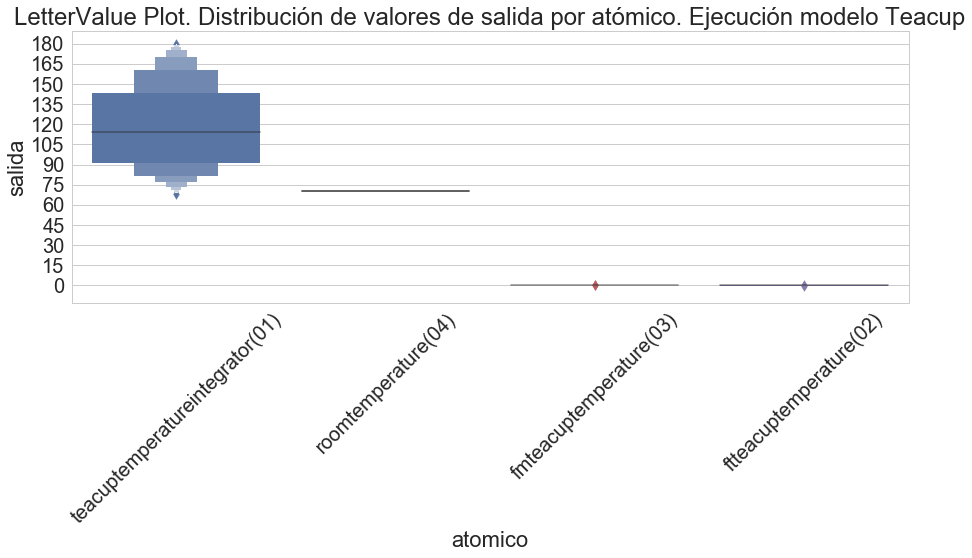
\includegraphics[scale=0.4]{imagenes/tea_output_letter_plot}}
        \caption{Modelo teacup - comportamiento estructural}
\end{figure}


Aplicamos la misma técnica para el análisis estructural del modelo \textit{SIR} traducido.
En la figura \ref{fig:sir_cant_mensajes} podemos observar los distintos modelos
que interactúan en el modelo así como la cantidad de mensajes que envían por
cada tipo.
Por cómo está estructurado el modelo, se observa nuevamente que la cantidad de
mensaje de tipo \textit{*, @} coincide para los modelos relacionados con la
integración. 

\begin{figure}[H]
	\centering     %%% not \center
	\subfigure[Cantidad mensajes modelo SIR]{\label{fig:sir_cant_mensajes}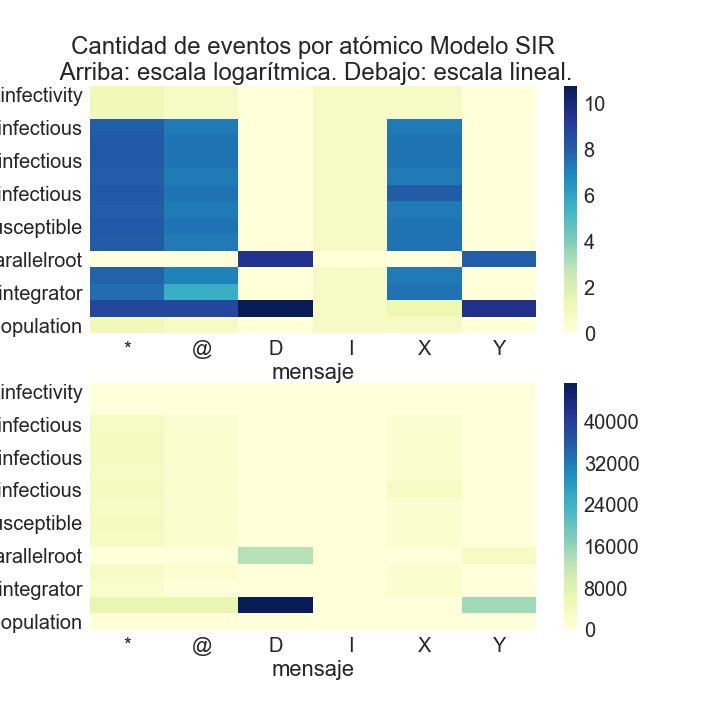
\includegraphics[scale=0.4]{imagenes/sir_cantidad_mensajes}}
	\subfigure[Valores de salida atómicos modelo SIR]{\label{fig:sir_output_letter_plot}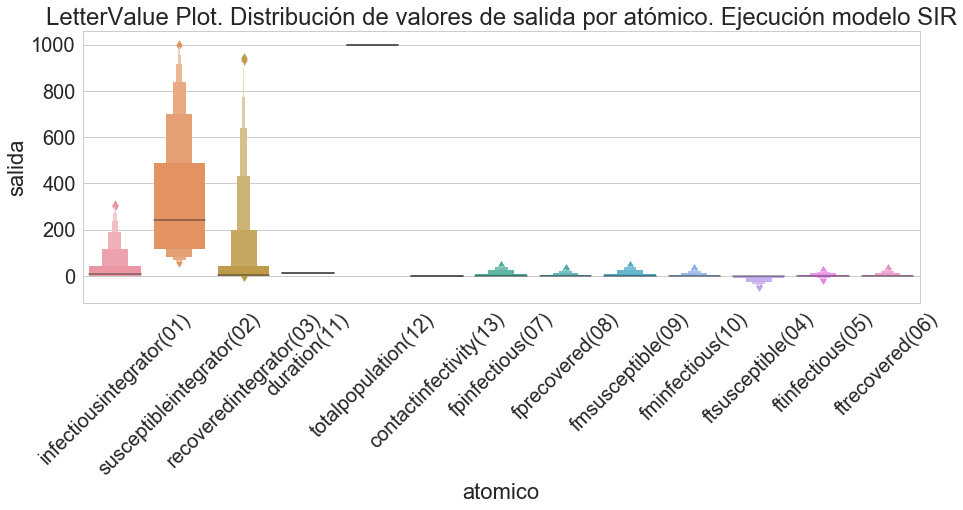
\includegraphics[scale=0.4]{imagenes/sir_output_letter_plot}}
        \caption{Modelo SIR - comportamiento estructural}
\end{figure}
